% 2016 年全国卷Ⅱ文科第 19 题：菱形与折叠后的五棱锥示意图
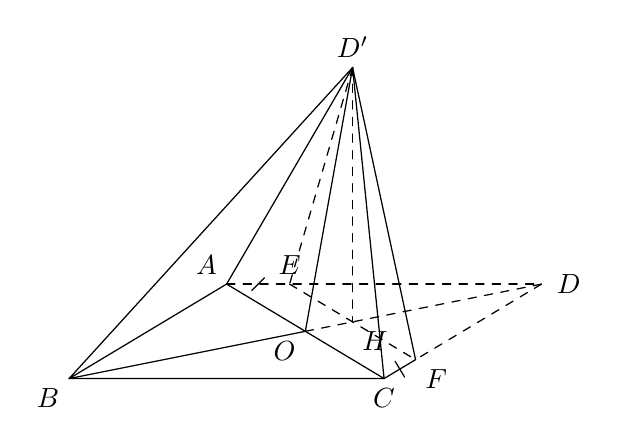
\begin{tikzpicture}[line width=0.45pt, line cap=round, line join=round]
  \coordinate (A) at (0,1.2);
  \coordinate (B) at (-2,0);
  \coordinate (C) at (2,0);
  \coordinate (D) at (4,1.2);
  \coordinate (O) at (1,0.6);
  \coordinate (E) at (0.8,1.2);
  \coordinate (F) at (2.4,0.24);
  \coordinate (H) at (1.6,0.72);
  \coordinate (Dp) at (1.6,3.95);

  % 菱形的后侧边及被遮挡的底面线段。
  \draw[dashed] (A) -- (D);
  \draw[dashed] (D) -- (F);
  \draw[dashed] (E) -- (H) -- (F);
  \draw[dashed] (O) -- (H) -- (D);

  % 菱形前侧边、对角线 AC 及可见的 BD 段。
  \draw (A) -- (B) -- (C) -- (F);
  \draw (A) -- (O) -- (C);
  \draw (B) -- (O);

  % 折起顶点 D' 与图中可见的棱、辅助连线。
  \draw (Dp) -- (A);
  \draw (Dp) -- (B);
  \draw[dashed] (Dp) -- (E);
  \draw (Dp) -- (O);
  \draw[dashed] (Dp) -- (H);
  \draw (Dp) -- (C);
  \draw (Dp) -- (F);

  % AE=CF 的等长记号。
  \draw (0.32,1.12) -- (0.48,1.28);
  \draw (2.14,0.22) -- (2.26,0.02);

  \node[above] at (Dp) {$D'$};
  \node[above left] at (A) {$A$};
  \node[below left] at (B) {$B$};
  \node[below] at (C) {$C$};
  \node[right=2pt] at (D) {$D$};
  \node[above] at (E) {$E$};
  \node[below right] at (F) {$F$};
  \node[below left] at (O) {$O$};
  \node[below right] at (H) {$H$};
\end{tikzpicture}
